\documentclass[../main.tex]{subfiles}

\begin{document}
As a goal to accelerate electrons in the LWFA scheme using gas--filled capillaries, we demonstrated a working set--up to produce jitter controlled plasma discharges in straight capillaries, achieving control on the time scale of
\begin{equation*}
    	\tau_\text{jitter}\approx 1\pm 0.36\si{\ns}.
\end{equation*}
%The primary motivation is to guide a high intensity short laser pulse,
The time window for which optical guiding exists was found, using a \SI{800}{\nm} oscillator laser, to be $\sim$\SI{350}{\ns} after the plasma ignition, and to last \SIrange{50}{100}{\ns}. A maximum radiation transmittance of 6.7 was observed.

Formation of the plasma channel for the straight capillary was cross--checked by spectroscopy measurements. We observed radial parabolic density profile channel with an increase in the electron density of $$\Delta N_e =\SI{0.4e18}{\per\cubic\cm}$$ and radius
$$r_\text{ch}\approx \SI{50}{\um}$$ with on-axis electron density $$N_e(0)=\SI{0.4e18}{\per\cubic\cm}.$$
The mean plasma density across the longitudinal capillary dimension was found to be \SI{2.7e17}{\per\cubic\cm}.

When experimenting with a curved capillary, we couldn't repeat the same result of optical guiding with the laser pulse--train. We shall now give some explanations to why we failed.

\begin{figure}
    \centering
    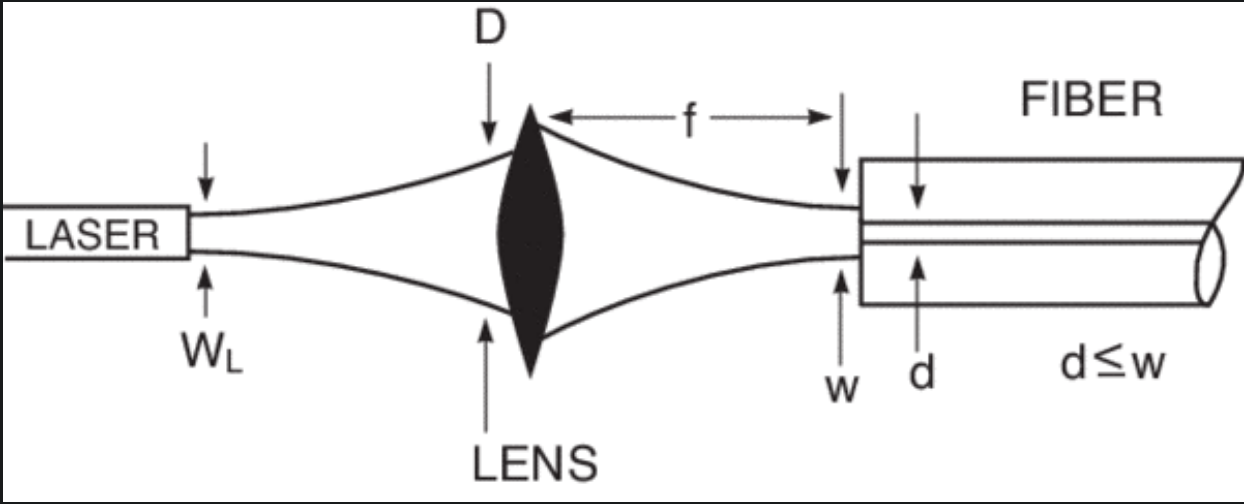
\includegraphics[width=\textwidth]{figures/Curved capillaries/coupling light to fiber.PNG}
    \caption{\href{https://www.newport.com/t/fiber-optic-basics}{From here.}}
    \label{fig:fiber}
\end{figure}

\end{document}